\begin{figure}[H]
  \centering
  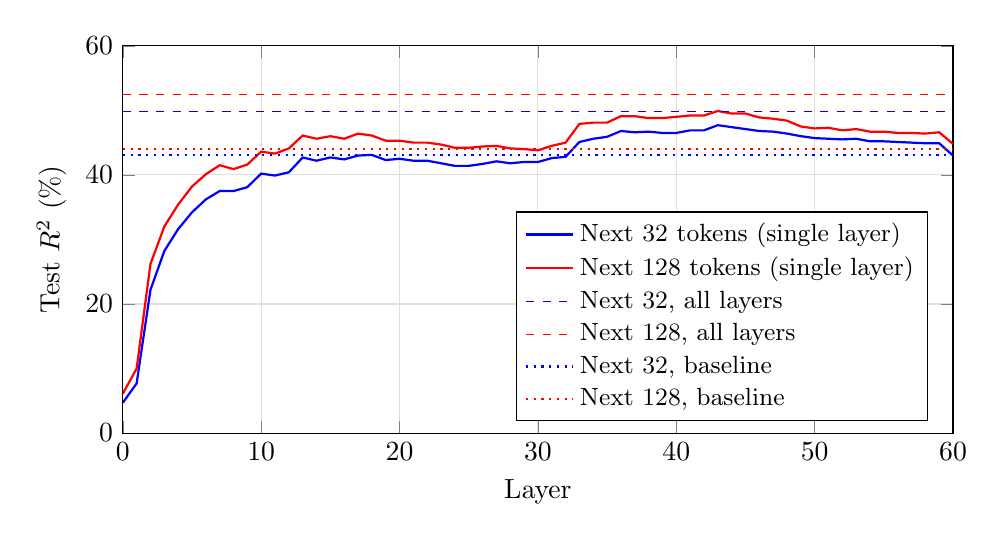
\begin{tikzpicture}
    \begin{axis}[
        width=\linewidth, height=6.5cm,
        xlabel={Layer}, ylabel={Test $R^2$ (\%)},
        xmin=0, xmax=60, ymin=0, ymax=60,
        xtick={0,10,20,30,40,50,60},
        grid=major, grid style={gray!25},
        legend pos=south east, legend cell align=left,
        legend style={font=\small},
      ]
      \addplot[thick, blue, mark=none] coordinates {
        (0,4.7) (1,7.7) (2,22.2) (3,28.2) (4,31.6) (5,34.2) (6,36.2) (7,37.5) (8,37.5) (9,38.1)
        (10,40.2) (11,39.9) (12,40.4) (13,42.7) (14,42.2) (15,42.7) (16,42.4) (17,43.0) (18,43.1) (19,42.3)
        (20,42.5) (21,42.2) (22,42.2) (23,41.8) (24,41.4) (25,41.4) (26,41.7) (27,42.1) (28,41.8) (29,42.0)
        (30,42.0) (31,42.6) (32,42.8) (33,45.1) (34,45.6) (35,45.9) (36,46.8) (37,46.6) (38,46.7) (39,46.5)
        (40,46.5) (41,46.9) (42,46.9) (43,47.7) (44,47.4) (45,47.1) (46,46.8) (47,46.7) (48,46.4) (49,46.0)
        (50,45.7) (51,45.6) (52,45.5) (53,45.6) (54,45.2) (55,45.2) (56,45.1) (57,45.0) (58,44.9) (59,44.9)
        (60,43.0)
      };
      \addlegendentry{Next 32 tokens (single layer)}
      \addplot[thick, red, mark=none] coordinates {
        (0,6.1) (1,10.0) (2,26.2) (3,32.0) (4,35.4) (5,38.2) (6,40.1) (7,41.5) (8,40.9) (9,41.6)
        (10,43.6) (11,43.3) (12,44.1) (13,46.1) (14,45.6) (15,46.0) (16,45.6) (17,46.4) (18,46.1) (19,45.3)
        (20,45.3) (21,45.0) (22,45.0) (23,44.7) (24,44.2) (25,44.2) (26,44.4) (27,44.5) (28,44.1) (29,44.0)
        (30,43.8) (31,44.5) (32,45.0) (33,47.9) (34,48.1) (35,48.1) (36,49.1) (37,49.1) (38,48.8) (39,48.8)
        (40,49.0) (41,49.2) (42,49.2) (43,49.9) (44,49.5) (45,49.5) (46,48.9) (47,48.7) (48,48.4) (49,47.5)
        (50,47.2) (51,47.3) (52,46.9) (53,47.1) (54,46.7) (55,46.7) (56,46.5) (57,46.5) (58,46.4) (59,46.6)
        (60,44.8)
      };
      \addlegendentry{Next 128 tokens (single layer)}
      \addplot[blue, dashed] coordinates {(0,49.8) (60,49.8)};
      \addlegendentry{Next 32, all layers}
      \addplot[red, dashed] coordinates {(0,52.4) (60,52.4)};
      \addlegendentry{Next 128, all layers}
      \addplot[blue, dotted, thick] coordinates {(0,43.1) (60,43.1)};
      \addlegendentry{Next 32, baseline}
      \addplot[red, dotted, thick] coordinates {(0,44.0) (60,44.0)};
      \addlegendentry{Next 128, baseline}
    \end{axis}
  \end{tikzpicture}
  \caption{Test $R^2$ for predicting difficulty (mean surprisal of the next 32 or 128 tokens after the next one) from a linear probe on one layer's activations at the current token. Dashed: one probe on all 61 layers. Dotted: text-statistics baseline. Single layers peak at layer 43 (32) and 43 (128).}
  \label{fig:layer-r2}
\end{figure}
